\documentclass[%
 aps,%
 pra,%
 preprint, %
 %tightenlines % use this to make the document single-spaced
 amsmath, % defines some math structures (ams is the American Mathematical Society)
 amsfonts, % load some fonts
 amssymb, % defines some mathematical symbols
]{revtex4-2}


\usepackage{graphicx}% Needed to include figure files
\usepackage{dcolumn}% Allows tables to align columns on the decimal point


% Here is a place to define symbols or commands that you use often, but which are not standard
\newcommand\half{\frac{1}{2}} %
\newcommand{\scientific}[2]{$#1 \times 10^{#2}$}
\newcommand*{\ket}[1][\psi]{|#1\rangle}
\newcommand{\D}{Deuterium}
\newcommand{\Rin}{$R_\infty$ }
\newcommand{\comment}[1]{}
\begin{document}

% These are the "Frontmatter Commands"

\title{Determination of $R_{\infty}$ and the \D-to-Proton mass ratio through Optical Spectroscopy}
\thanks{Professor Conover for Providing Data and Guidance throughout the whole process}% Thanks gives a footnote to the article title

\author{Adithya Shastry} % Note that Tex puts a double space after each period; "~" suppressed that
\email[Author to whom correspondence should be addressed: ]{amshas21@colby.edu}%



\affiliation{Colby College\\ Waterville, ME }% Force a line break with "\\"


\date{\today}% It is always \today, today, but you should enter the date of submission in this spot




\begin{abstract}  % insert abstract here
Using the methods of optical spectroscopy the \Rin and the \D-to-proton mass ratio were measured with high degrees of accuracy.Measurements were made on the Balmer series transition wavelengths of Hydrogen and \D  atoms in a specially made \D  lamp which contained more than the the natural abundance of Hydrogen's Isotope. \Rin was measured at $R_{\infty}=10975000 \pm 1000 \text{m}^{-1}$ and \D-to-proton mass ratio,$\frac{m_d}{m_p}$, was measured at $\frac{m_d}{m_p}=2.0 \pm 0.2$ which gives a percent uncertainty of 0.012\% and 0.882\% respectively. 
\end{abstract}


\maketitle 

\newpage

\section{\label{sec:OpticalSpec} Introduction: Optical Spectroscopy of Hydrogen and \D }
Optical spectroscopy is a method of measuring the spectrum of atomic light emissions of an atom as they return to their respective $n=2$ states. With an optical spectrometer, this can be done to a high degree of accuracy and precision. For this reason the methods of optical spectroscopy have provided the foundations for the development of quantum mechanics as a field of study. Through the optical spectrometer, we are able identify identify fundamental quantities such as the Rydberg Constant for different atoms and, even know what a material is made of through understanding what spectrum it emits. \Rin is a fundamental quantity that is used to understand the energy levels of atoms of very heavy elements but can be adapted, as explained below, to be applied to relatively less massive atoms as well\cite{Eisberg1985}.Since \Rin is among the most accurately measured physical constants it is a great candidate to test the ability of optical spectroscopy to make accurate wavelength measurements at the quantum scale. The \D-to-Proton mass ratio gives the ratio of Hydrogen's less abundant isotope, \D , which has a neutron in its nucleus and a proton. 

Through the use of optical spectroscopy, we will attempt to measure $R_\infty$ and the \D-to-Proton mass ratio by using measurements of the Balmer series emission wavelengths of both Hydrogen and \D. The Balmer series are the transitions of excited electrons of $n_i>2$ states to the $n_f=2$ state\cite{Eisberg1985}. The energy levels of the Hydrogen atom are shown in the following equation\cite{Eisberg1985}:
\begin{equation}
    \label{Eq:EnergyLevels}
    E_n=-\frac{1}{2}\mu c^2 (Z\alpha)^2 \frac{1}{n^2}
\end{equation}
Where $\alpha$ is given by 
\begin{equation}
    \alpha=\frac{e^2}{4\pi \epsilon_0 \hbar c}\approx \frac{1}{137}\cite{CODATA2020}
\end{equation}
and $\mu$ is the reduced mass given by 
\begin{equation}
    \mu=\frac{m_em_N}{m_e+m_N}
\end{equation}


Through some derivation, which can be seen in Appendix \ref{app:DerivationsI} and \ref{app:DerivationsII}, we can derive the equations we need to measure the $R_\infty$ and the \D-to-Proton mass ratio, $\frac{m_d}{m_p}$. The equations for the measurement of $R_\infty$ are shown below. First we will first start with measuring $R_H$ from which $R_\infty$ can be derived. \Rin is the Rydberg constant for an atom of infinite mass, and $R_H$ is the Rydberg constant for Hydrogen. 
\begin{equation}
\label{Eq:RH}
    \frac{1}{\lambda_{H_{i-f}}}=R_H\xi_{i-f}
\end{equation}
Where $\xi_{i-f}$ is given by
\begin{equation}
    \label{Eq:xi}
    \xi_{i-f}=\frac{n_i^2-n_f^2}{n_i^2n_f^2}
\end{equation}{}
With this $R_H$ value, we can then find $R_\infty$ by using the following formula
\begin{equation}
\label{Eq:Rinf}
    R_\infty=F_HR_H
\end{equation}{}
Where $F_H=1+\frac{m_e}{m_N}=1+0.000544617=1.000544617$ \cite{CODATA2020}. As seen in Equation \ref{Eq:Rinf} the two types of Rydberg constants are very closely related to one-another (Through the $F_H$ constant.)

In order to measure the \D-to-proton mass ratio we will use the equation below. 
\begin{equation}
    \label{Eq:md-mp}
    \frac{m_d}{m_p}=\frac{A_{i-f}}{A_{i-f}-\Delta\lambda_{i-f}}
\end{equation}{}
Where $\Delta\lambda_{i-f}=\lambda_{H_{i-f}}-\lambda_{D_{i-f}}$ and $A_{i-f}=\lambda_{H_{i-f}}-\lambda_{\infty_{i-f}}$. The equation for $\lambda_{\infty_{i-f}}$ is given below:
\begin{equation}
    \lambda_{\infty_{i-f}}=\frac{1}{R_\infty \xi_{i-f} }
\end{equation}{}


\section{\label{sec:Experiment} Experiment}
The experiment will be conducted using the Horiba 1250M-II spectrometer. This Spectrometer is very good at finding wavelengths at a very precise scale, but because the measurements are so precise the Spectrometer is greatly affected by the environment it is in. For example, a small change in the ambient temperature of the lab can have a significant affect on the accuracy of the wavelengths being measured. However, the spectrometer has very little trouble measuring wavelength differences since those measurements are both subject to the same offset(as a result of the environment the spectrometer is in and other factors). For this reason, the \D-to-Proton mass ratio measurements will be significantly more accurate since it relies on a measured difference in the peak wavelengths for Hydrogen and \D. To account for this systematic, yet random, error, a correction factor was calculated and implemented to the data as seen in Appendix \ref{app:Error}. This issue of accuracy will be further presented in Table \ref{tab:Raw Data}

Since the overall abundance of \D   is around 0.015\%, we would not be able to measure the \D   spectral lines with a normal Hydrogen lamp. To account for this, a \D   lamp was used during the experimentation procedures. With this the $\alpha$,$\beta$,$\gamma$,$\delta$,and $\epsilon$ spectral lines were measured of Hydrogen and \D   using the spectrometer and the instructions specific to it. The spectra were then analysed using excel and the peaks were manually picked out and analysed later. An example of such spectra can be seen in Figure \ref{fig:Spectrum}

\begin{figure}[h!]
  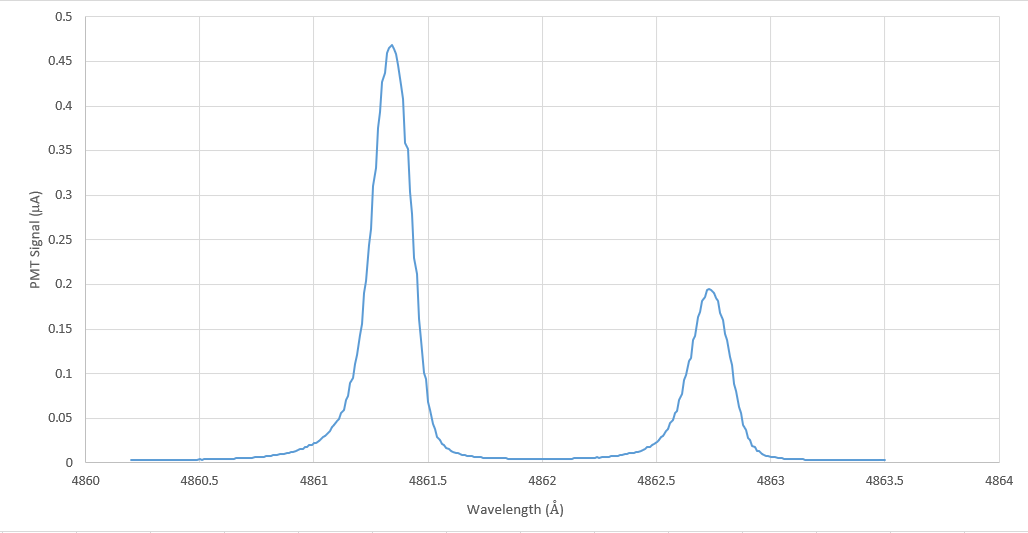
\includegraphics[width=\linewidth]{Figures/Spectral.PNG}
  \caption{This is the Experimental Spectra of $H_{\beta}$ and $D_{\beta}$ from which the peaks were derived and analysed later.}
  \label{fig:Spectrum}
\end{figure}
\newpage


\section{\label{sec:Results} Results}
As discussed in section \ref{sec:Experiment}, the data was collected by examining figures like Figure \ref{fig:Spectrum} for the Balmer series spectra that were measured. 
\begin{table}[]
\begin{tabular}{l|l|l|l|l}
\hline 
\hline
$n_i$ & $\lambda_{H_{i-f}}$(nm) & $\sigma_{\lambda_H}$(nm) & $\lambda_{D_{i-f}}$(nm) & $\sigma_{\lambda_D}$(nm)\\
\hline
3     & 656.423               & 0.002                    & 656.250               & 0.002                    \\
4     & 486.270               & 0.002                    & 486.140               & 0.002                    \\
5     & 434.170               & 0.002                    & 434.050               & 0.001                    \\
6     & 410.290               & 0.003                    & 410.170               & 0.002                    \\
7     & 397.140               & 0.003                    & 397.030               & 0.001                    \\
8     & 389.020               & 0.003                    & 388.920               & 0.002 \\
\hline
\hline
\end{tabular}
\label{tab:Raw Data}
\caption{This shows the raw data that was extracted from the spectroscopic graphs as described in Section \ref{sec:Experiment}}
\end{table}
\newpage
The uncertainty in the wavelength peak measurements shows more clearly what was previously discussed. The spectrometer is very much capable of measuring wavelengths precisely, but because of external factors, it tends to not measure these wavelengths very accurately.  

Based on previous usage of this spectrometer, it is clear that the measurements made by the spectrometer were in fact not in alignment with the accepted wavelengths for the different transitions. After some analysis, the correction factor for single wavelength measurements was noted as $-0.13\pm 0.02$ nm(Please refer to Appendix \ref{app:Error} to see the method that was used to obtain this correction). This was then applied to all of the measurements listed in Table \ref{tab:Raw Data}. This correction should rectify accuracy issue in the measurement of the wavelengths. The wavelength measurements made in air were then converted to vacuum measurements since all of the formulas shown in Section \ref{sec:OpticalSpec} deal with wavelengths in vacuum. This can be done using the Equation \ref{Eq:vac}.
\begin{equation}
    \label{Eq:vac}
    \lambda_{\text{vacuum}}=\lambda_{\text{air}}n_{air}
\end{equation}{}
These corrected measurements can be seen in Table \ref{tab:corrected}
\begin{table}[h!]
\begin{tabular}{lllll}
\hline
\hline
\multicolumn{5}{c}{Corrected Data}                                                                                                                                                             \\ \hline
\multicolumn{1}{l|}{$n_i$} & \multicolumn{1}{l|}{$\lambda_{H_{i-f}}$(nm)} & \multicolumn{1}{l|}{$\sigma_{\lambda_H}$(nm)} & \multicolumn{1}{l|}{$\lambda_{D_{i-f}}$(nm)} & $\sigma_{\lambda_D}$(nm) \\
\hline
\multicolumn{1}{l|}{3}     & \multicolumn{1}{l|}{656.29}                & \multicolumn{1}{l|}{0.02}                    & \multicolumn{1}{l|}{656.120}                & 0.02                   \\
\multicolumn{1}{l|}{4}     & \multicolumn{1}{l|}{486.14}                & \multicolumn{1}{l|}{0.02}                    & \multicolumn{1}{l|}{486.010}                & 0.02                   \\
\multicolumn{1}{l|}{5}     & \multicolumn{1}{l|}{434.04}                & \multicolumn{1}{l|}{0.02}                    & \multicolumn{1}{l|}{433.920}                & 0.02                   \\
\multicolumn{1}{l|}{6}     & \multicolumn{1}{l|}{410.16}                & \multicolumn{1}{l|}{0.02}                    & \multicolumn{1}{l|}{410.040}                & 0.02                   \\
\multicolumn{1}{l|}{7}     & \multicolumn{1}{l|}{397.01}                & \multicolumn{1}{l|}{0.02}                    & \multicolumn{1}{l|}{396.900}                & 0.02                   \\
\multicolumn{1}{l|}{8}     & \multicolumn{1}{l|}{388.89}                & \multicolumn{1}{l|}{0.02}                    & \multicolumn{1}{l|}{388.790}                & 0.02          \\
\hline
\hline
\end{tabular}
\caption{
This table shows the data from Table \ref{tab:Raw Data} corrected for the offset in wavelength measurement and converted to vacuum wavelength measurements using Equation \ref{Eq:vac}}
\label{tab:corrected}
\end{table}
\newpage











\section{\label{sec:Discussion} Discussion}
The analysis will be done in two sections corresponding to the initial purpose of the experiment: determining the $R_\infty$ and determining the \D-to-proton mass ratio. This will utilize the equations laid out in Section \ref{sec:OpticalSpec}(The derivations for which can be seen in Appendix \ref{app:DerivationsI} and \ref{app:DerivationsII}). 



\subsection{\label{sec:Rinf}Determining $R_\infty$}

The central equations that will be used to determine the \Rin  are Equations \ref{Eq:RH} and \ref{Eq:Rinf}. $R_H$ was determined by doing a linear regression with respect to Equation \ref{Eq:RH} using the corrected data seen in Table \ref{tab:corrected} and the calculated values for $\xi_{i-f}$ using Equation \ref{Eq:xi}. This calculation can be seen in Table \ref{tab:RH}.
\begin{table}[]
\begin{tabular}{c|r|r}
\hline
\hline
$n_i$ & \multicolumn{1}{l|}{$\xi_{i-f}$} & \multicolumn{1}{l}{$\frac{1}{\lambda_{i-f}}(\text{nm}^{-1})$} \\ \hline
3     & 0.139                            & 0.0015                                                        \\
4     & 0.188                            & 0.0021                                                        \\
5     & 0.210                            & 0.0023                                                        \\
6     & 0.222                            & 0.002                                                         \\
7     & 0.230                            & 0.003                                                         \\
8     & 0.234                            & 0.002                                                         \\ 
\hline
\hline
\end{tabular}
\caption{This table contains the data used to determine the value of $R_H$ using linear regression. $\xi_{i-f}$ is a calculated unit-less value that was calculated using Equation \ref{Eq:xi}. Notice that the table is plotting the inverse of the peaks measured in Table \ref{tab:corrected}}
\label{tab:RH}
\end{table}
\newpage
A plot of this data can be seen in Figure \ref{fig:LinearRegression}

\begin{figure}[h!]
  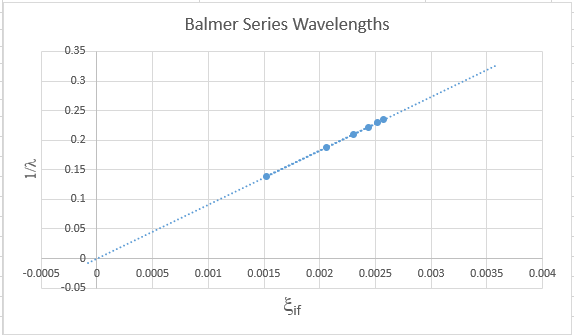
\includegraphics[scale=1]{Figures/LinearRegression.PNG}
  \caption{This Figure shows a plot of the data shown in Table \ref{tab:RH} in accordance with Equation \ref{Eq:RH}.$R_H$ can be derived from the slope of this line}
  \label{fig:LinearRegression}
\end{figure}
\newpage
 The linear regression of this data provided us with results which can be seen in Table \ref{tab:linear}

\begin{table}[]
\begin{tabular}{ll}
\hline
\hline
\multicolumn{2}{c}{Linear Regression Results} \\ \hline
\multicolumn{1}{l|}{$R_H\text{nm}^{-1}$} & Intercept \\
\multicolumn{1}{l|}{$0.010969062 \pm$  \scientific{6.12423}{-7}} & \scientific{-2.07756}{-7}$ \pm$ \scientific{1.26396}{-7} \\ \hline
\hline
\end{tabular}
\caption{This table shows the results of the linear regression done on the data in Table \ref{tab:RH}}
\label{tab:linear}
\end{table}
\newpage
As can be seen in Table \ref{tab:linear}, the linear regression did pick up an intercept.However, given the error associated with the intercept and the fact it is not noticeable in Figure \ref{fig:LinearRegression}, we can essentially disregard it. The error of the $R_H$ measurement, as can be seen in the table, is very small compared to the value measured. This again shows the precision with which the Horiba spectrometer measures optical spectra. The final step is to convert the $R_H$ data to \Rin  using Equation \ref{Eq:Rinf}. This results in a $R_\infty=10975000 \pm 1000\text{m}^{-1}$. The \Rin  value was converted to $\text{m}^{-1}$ from $\text{nm}^{-1}$ in order to have the same units as the the accepted value of $R_\infty=10973731.57$\cite{CODATA2020}. This means there is a percent difference of $0.012\%$ from the accepted value. This,again, shows that optical spectroscopy can produce very accurate and precise results for these sorts of spectral measurements. 


\subsection{Determining the \D-to-proton mass ratio, $\frac{m_d}{m_p}$}
To determine $\frac{m_d}{m_p}$ the main equation that will be used is Equation \ref{Eq:md-mp}. This has been done in Table \ref{tab:md-mp}(The error propagation done in this table will be explained in Appendix \ref{app:Error}).

\begin{table}[]
\begin{tabular}{l|l|l|l|l}
\hline
\hline
$n_i$ & $A_{i-f}$   & $\Delta \lambda$ & $\sigma_{\Delta \lambda}$ & $\frac{m_d}{m_p}$ \\ \hline
3  & 0.3573299   & 0.173      & 0.003              & 1.939036941       \\
4  & 0.264688815 & 0.130       & 0.003              & 1.965711445       \\
5  & 0.236329299 & 0.120      & 0.002               & 2.032132967       \\
6  & 0.223331187 & 0.120       & 0.004              & 2.162007413       \\
7  & 0.216162532 & 0.110       & 0.003              & 2.036729561       \\
8  & 0.211751052 & 0.100        & 0.004              & 1.895314265       \\ \hline
\hline
\end{tabular}
\caption{This table shows the calculation of $\frac{m_d}{m_p}$ using Equation \ref{Eq:md-mp} and its parts.}
\label{tab:md-mp}
\end{table}
With this data a weight was calculated based on the error of the $\Delta \lambda$, $\sigma_{\Delta \lambda}$, as seen in Table \ref{tab:md-mp}(The process that determined the weights of each measurement will be described in Appendix \ref{app:Error}). The Weighted Average of the $\frac{m_d}{m_p}$ measurements gave a final result of $\frac{m_d}{m_p}=2.0 \pm 0.2$. The accepted value is $\frac{m_d}{m_p}=1.99900750139$\cite{CODATA2020}. This gives a percent error of $0.882\%$ which, as in the case of the \Rin, is very small. This shows the Spectrometer's ability to measure wavelength differences with great precision since the correction factor will have no affect on the wavelength difference calculation, $\sigma_{\Delta \lambda}$ will be greatly affected by any systematic errors in the spectrometer itself. 

\section{Conclusion}
From these two experiments, it is quite clear why optical spectroscopy is so widely used in the fields of experimental physics and quantum mechanics. The precision and accuracy of the measurements of \Rin and the \D-to-Proton mass ratio prove that the spectrometer can be used to measure other atomic data as well as rigorously test quantum mechanical theories.










% Acknowledgements appear at the end of the paper as an unnumbered section.
\begin{acknowledgments}
I would like to thank Professor Conover for conducting the experiment, providing me the data, and helping me analyze the data as well as write the report. 
\end{acknowledgments}















% Specify following sections are appendices. Use \appendix* if there
% only one appendix.
\appendix
\section{\label{app:DerivationsI} Derivations For $ R_{\infty}$}
The derivation of the equation for $R_H$, Equation \ref{Eq:RH} can be done by starting with Equation \ref{Eq:EnergyLevels}. A lot of these constants are combined and written as $R_N$, the Rydberg constant. The equation for the energy levels then takes the form 
\begin{equation}
\label{Eq:En}
    E_n=-\frac{hcR_N}{n^2}
\end{equation}{}
With Equation \ref{Eq:En}, we can derive Equation \ref{Eq:RH}. This will be done below
\begin{align*}
\Delta E_{N_i-f}&=E_{N_i}-E_{N_f}\\
&=hcR_N(\frac{1}{n_f^2}-\frac{1}{n_{i}^2})\\
&=hcR_N(\frac{n_i^2-n_f^2}{n_i^2n_f^2})\\
&=hcR_N\xi_{i-f}
\end{align*}












This can then be converted to a wavelength equation using the following relation
\begin{equation}
    \label{VaccWavePhot}
    \lambda_{N_{i-f}}=\frac{hc}{\Delta E_{N_{i-f}}}
\end{equation}{}
Substituting the into Equation \ref{VaccWavePhot} and solving for $\lambda_{N_{i-f}}$ leads us to
\begin{equation}
\label{Eq:finalstep}
    \lambda_{N_{i-f}}=\frac{1}{R_N\xi_{i-f}}
\end{equation}{}
Using the relationship between \Rin  and $R_N$ given by Equation \ref{Eq:FN}
\begin{equation}
    \label{Eq:FN}
    R_\infty=F_NR_N
\end{equation}{}
We can get the following, where instead of using $R_N$, we can use \Rin . Which is a cool result that shows that the wavelengths of the emission spectra can be described by \Rin  and does not necessarily have to rely on $R_N$.
\begin{equation}
\label{Eq:lambdaN}
\lambda_{N_{i-f}}=\frac{F_N}{R_\infty\xi_{i-f}}
\end{equation}{}
This is not the final result we want. To get the final result that we want, Equation \ref{Eq:RH}, we can simply restrict Equation \ref{Eq:finalstep} to only work for Hydrogen by using $R_H$ instead of $R_N$. This can be seen in Equation \ref{Eq:Final}
\begin{equation}
\label{Eq:Final}
    \frac{1}{\lambda_{H_{i-f}}}=R_H\xi_{i-f}
\end{equation}{}
























\section{\label{app:DerivationsII} Derivations For $\frac{m_d}{m_p}$}
We can derive the equation for $\frac{m_d}{m_p}$ by starting from Equation \ref{Eq:lambdaN}. First, we can slightly modify this equation by considering what $F_N$ will be if we had a nucleus with infinite mass. When this is the case $F_N \approx 1$, when we substitute this fact into Equation \ref{Eq:lambdaN} we get the following:
\begin{equation}
\label{Eq:LambdaInf}
    \lambda_{\infty_{i-f}}=\frac{1}{R_\infty\xi_{i-f}}
\end{equation}{}
With this equation in mind, we can now solve for the Equation \ref{Eq:md-mp} from Equation \ref{Eq:LambdaInf} and \ref{Eq:lambdaN}. This will be done below:
\begin{align*}
    \lambda_{H_{i-f}}-\lambda_{\infty_{i-f}}&=\frac{F_N}{R_\infty\xi_{i-f}}-\frac{1}{R_\infty\xi_{i-f}}\\
    &=\frac{F_H-1}{R_\infty\xi_{i-f}}
\end{align*}{}
Now recall, that $F_N=1+\frac{m_e}{m_N}$. Since Hydrogen only has one proton, the mass of the nucleus is just the mass of the proton. That is, $F_H=1+\frac{m_e}{m_p}$. We can plug this into the equation above in order to get the following:
\begin{equation}
    \label{Eq:lambdaH-lambdainf}
    \lambda_{H_{i-f}}-\lambda_{\infty_{i-f}}=\frac{F_H-1}{R_\infty\xi_{i-f}}=\frac{m_e}{m_p}\frac{1}{R_\infty\xi_{i-f}}
\end{equation}{}
Now the same can be done for \D, but instead $F_D=1+\frac{M_e}{m_d}$, since \D atom doesn't only have a mass of one proton. This leads us to the following
\begin{align*}
    \lambda_{D_{i-f}}-\lambda_{\infty_{i-f}}&=\frac{F_D}{R_\infty\xi_{i-f}}-\frac{1}{R_\infty\xi_{i-f}}\\
    &=\frac{F_D-1}{R_\infty\xi_{i-f}}\\
    &=\frac{m_e}{m_d}\frac{1}{R_\infty\xi_{i-f}}
\end{align*}{}
\begin{equation}
    \label{Eq:lambdaD-lambdainf}
    \lambda_{D_{i-f}}-\lambda_{\infty_{i-f}}=\frac{m_e}{m_d}\frac{1}{R_\infty\xi_{i-f}}
\end{equation}{}
When we take the ratio of Equations \ref{Eq:lambdaH-lambdainf} and \ref{Eq:lambdaD-lambdainf} we get the following:
\begin{equation}
    \label{Eq:lambdaRatio-Md-MP}
    \frac{\lambda_{H_{i-f}}-\lambda_{\infty_{i-f}}}{\lambda_{D_{i-f}}-\lambda_{\infty_{i-f}}}=\frac{m_d}{m_p}
\end{equation}{}
With Equation \ref{Eq:lambdaRatio-Md-MP} we can derive Equation \ref{Eq:md-mp} with some clever definitions and manipulations.
\begin{align*}
    \frac{m_d}{m_p}&=\frac{\lambda_{H_{i-f}}-\lambda_{\infty_{i-f}}}{\lambda_{D_{i-f}}-\lambda_{\infty_{i-f}}}\\
    \intertext{First let us define $A_{i-f}=\lambda_{H_{i-f}}-\lambda_{\infty_{i-f}}$}\\
    &=\frac{A_{i-f}}{\lambda_{D_{i-f}}-\lambda_{\infty_{i-f}}}\\
    \intertext{Let is add and subtract $\lambda_{H_{i-f}}$}\\
    &=\frac{A_{i-f}}{\lambda_{D_{i-f}}+(\lambda_{H_{i-f}}-\lambda_{H_{i-f}})-\lambda_{\infty_{i-f}}}\\
    \intertext{Let's do a bit of rearranging and then substitute in $A_{i-f}$}\\
    &=\frac{A_{i-f}}{\lambda_{D_{i-f}}-\lambda_{H_{i-f}}+A_{i-f}}\\
\end{align*}{}
Now if we define $\Delta \lambda_{i-f}=\lambda_{H_{i-f}}-\lambda_{D_{i-f}}$ we will end up with Equation \ref{Eq:md-mp}
\begin{equation}
 \frac{m_d}{m_p}=\frac{A_{i-f}}{A_{i-f}-\Delta \lambda_{i-f}}
\end{equation}


















\section{\label{app:Error} Error Propagation Explanations}
Now we can discuss the various methods used to propagate error throughout the analysis process. This will be done in various sections
\subsection{Wavelength Measurements}
As stated in Section \ref{sec:Experiment} the data was read off of plots made in excel as seen in Figure \ref{fig:Spectrum}. The error when reading these plots was determined by looking at how spread out the peak of the graph was. For the most part the peaks of the various spectral lines had about a $\sigma \approx \pm 0.02$. 

\subsection{The correction factor}
The correction factor was determined by plotting various measurements made in a previous experiment, where we had ready access to the accepted wavelengths. The deviations from the norm were plotted as seen in Figure \ref{fig:correction} against the wavelength that they measured. 


\begin{figure}[h!]
  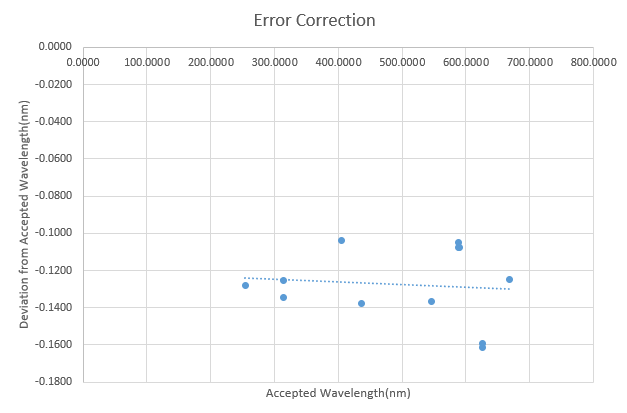
\includegraphics[width=\linewidth]{Figures/Correction.PNG}
  \caption{This is a plot of the deviation of the wavelength measurements from the accepted wavelength done in a previous experiment. This plot was used to estimate the correction factor $\sigma_c \approx -0.13 \pm 0.02$ nm}
  \label{fig:correction}
\end{figure}
\newpage




As can be seen in the graph, the correction factor was then estimated for around $\lambda=500$nm and was determined to be about $\sigma_c \approx -0.13 \pm 0.02$ nm.


\subsection{The Air to Vacuum Conversion}
For this conversion, the error was simply kept the same since the $n_{\text{air}} \approx 1$. This can be seen in Table \ref{tab:corrected}.

\subsection{Error Calculation for $\frac{m_d}{m_p}$ measurement}


From Table \ref{tab:md-mp} we can see that the error for $\sigma_{\lambda}$ was calculated in the standard way of dealing with uncertainties for addition and subtraction\cite{Taylor1997}. As mentioned in Section \ref{sec:Discussion}, a weighted average was taken to find the \D-to-Proton mass ratio. This process will be explained below.

\subsubsection{Calculating $\sigma_r$}
$\sigma_r$ gives us the error for the ratio being measured and was determined in the following way.
\begin{align*}
    \sigma_r&=\sqrt{(\frac{\partial r}{\partial \Delta \lambda_{i-f}})^2 \sigma_{\Delta_{\lambda}}}\\
    &=\frac{A_{i-f}}{(A_{i-f}-\Delta_{\lambda})^2} \sigma_{\Delta_{\lambda}}\\
\end{align*}{}
With this equation we can now calculate the weights. The way to calculate the weights must put less weight on the the values with a high $\sigma_r$. The best way to do this is to calculate the weights in the following way
\begin{equation}
    \label{Eq:weights}
    w_i=\frac{1}{\sigma_i^2}
\end{equation}{}
This was done for every measurement that we made. All of the above error propagation can be seen in Table \ref{tab:md-mp-error}



\begin{table}[]
\begin{tabular}{l|l|l|l}
\hline
\hline
$n_i$ & $\sigma_{\Delta \lambda}$ & $\sigma_{r}$ & $w_i=\frac{1}{\sigma_r^2}$ \\
\hline
3 & 0.028284271 & 0.029761019 & 1129.027177 \\
4 & 0.028284271 & 0.041290385 & 586.5460656 \\
5 & 0.02236068 & 0.039072543 & 655.0231401 \\
6 & 0.036055513 & 0.07546345 & 175.6008776 \\
7 & 0.031622777 & 0.060685693 & 271.5359712 \\
8 & 0.036055513 & 0.061165786 & 267.2901006\\
\hline
\hline
\end{tabular}
\caption{This table shows the error propagation for the \D-to-proton mass ratio measurement}
\label{tab:md-mp-error}
\end{table}
\newpage



Then a weighed average was taken using the standard formula seen in Equation \ref{Eq:WeightedAverage}\cite{Taylor1997}.
\begin{equation}
    \label{Eq:WeightedAverage}
    x_{\text{avg}}=\frac{\Sigma_{i=1}^N w_i x_i}{\Sigma_{i=1}^N w_i}
\end{equation}{}
The error is given by \ref{Eq:WeightedAverageError}\cite{Taylor1997}.
\begin{equation}
    \label{Eq:WeightedAverageError}
    \sigma_{\text{avg}}=\frac{1}{\sqrt{\Sigma_{i=1}^N w_i}}
\end{equation}{}
The weighted average and the uncertainty are shown in Section \ref{sec:Discussion}



\section{Thank you!}
Dear Professor Conover, 

I would like to thank you so much for a wonderful semester! I really wish things had gone differently and that I could have taken class with you in person, but such is life. I have really enjoyed every class I have taken with you and truly respect the amount of effort you put into every one of your classes. This has made me realize that to make something meaningful you must put in the effort. It has taken me most of my high school and college years to realize what I already knew when I was 10: that I wanted to be an Engineer. I now understand I wouldn't be truly happy in any other profession and for helping me come to this realization, I am truly grateful. I hope I get the opportunity to take the first step towards my dream this fall, but whatever may happen I know where my heart is and hope that it will guide me in the future.
\vspace{10mm}\\
Thank you so much Professor Conover!\\
Please stay safe!\\
Adi Shastry\\
(Sorry for the bad formatting)


\bibliographystyle{apsrev4-2}
\bibliography{./References/PH250Citations_Spring2020} 


\end{document}
